\documentclass[crop]{standalone}
\begin{document}

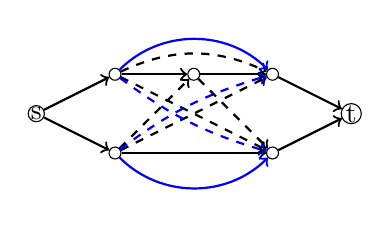
\begin{tikzpicture}
\tikzstyle{vertex}=[circle, draw, fill=white, inner sep=0pt, minimum width=1ex]
\tikzstyle{active-base-edge}=[->,black,thick]
\tikzstyle{inactive-base-edge}=[->,black,thick,dashed]
\tikzstyle{active-lifted-edge}=[->,blue,thick]
\tikzstyle{inactive-lifted-edge}=[->,blue,thick,dashed]
\node[style=vertex] (s) at (0,0) {s};
\node[style=vertex] (lu) at (1,0.5) {};
\node[style=vertex] (mu) at (2,0.5) {};
\node[style=vertex] (ru) at (3,0.5) {};
\node[style=vertex] (ll) at (1,-0.5) {};
\node[style=vertex] (rl) at (3,-0.5) {};
\node[style=vertex] (t) at (4,0) {t};

\draw[style=active-base-edge] (s) -- (lu);
\draw[style=active-base-edge] (lu) -- (mu);
\draw[style=active-base-edge] (mu) -- (ru);
\draw[style=active-base-edge] (ru) -- (t);

\draw[style=active-base-edge] (s) -- (ll);
\draw[style=active-base-edge] (ll) -- (rl);
\draw[style=active-base-edge] (rl) -- (t);

\draw[style=inactive-base-edge] (lu) -- (rl);
\draw[style=inactive-base-edge] (lu) to [bend left=25] (ru);
\draw[style=inactive-base-edge] (ll) -- (mu);
\draw[style=inactive-base-edge] (ll) -- (ru);
\draw[style=inactive-base-edge] (mu) -- (rl);

\draw[style=active-lifted-edge] (lu) to [bend left=45] (ru);
\draw[style=active-lifted-edge] (ll) to [bend right=45] (rl);
\draw[style=inactive-lifted-edge] (ll) to [bend left=10] (ru);
\draw[style=inactive-lifted-edge] (lu) to [bend right=10] (rl);

\end{tikzpicture}

\end{document}
